Before implementing an own solution, let's uncover some available and current implementations to this very problem. Naturally, big progress and research is performed in this topic, therefore this chapter is not meant to provide full market scan, or list every solution available. It rather aims to discover some fine examples of neural network implementations which perform well.

Later on you'll stumble upon a list of available face recognition databases and data sets, which can be used for training and evaluating our implementation. Each of the data set description is accompanied by a short list of their respective metrics.

\section{Existing CNN implementations}

There are many available solution and existing implementations\,\cite{face_rec}. They naturally differs, their models compete and cover different use cases\,\cite{handbook_face}. We have already established, that the face recognition is a dynamic field with competitive nature. Open challenges and competitions are enabling greater progress in the field. However that makes it impossible to provide an always up-to-date review of available solutions and implementations.

Here's a short list of example challenges and competitions held in the face recognition field. It provides an insight into how wide the field is and how many different architectures can be used:

\begin{itemize}
    \item MSCeleb challenges\,\footnote{\url{https://www.msceleb.org/celeb1m/1m} and \url{https://www.msceleb.org/challenge2/2017}}
    \item Deep learning benchmark\,\footnote{\url{https://github.com/u39kun/deep-learning-benchmark}}
    \item NIST: Fusion of Face Recognition Algorithms 2018\,\footnote{\url{https://www.nist.gov/programs-projects/fusion-face-recognition-algorithms-2018}}
    \item Surveillance Face Recognition Challenge\,\cite{sur_challenge}
\end{itemize}

Therefore let's rather focus on one single solution and pick some details of its design to better understand, how such implementation is made and what does it mean.

\subsection{FaceNet}
\label{ss:facenet}

This state-of-the-art solution backed by Google\,\cite{facenet} is one of the leading solutions in the field. Its implementation is open source\,\footnote{\url{https://github.com/davidsandberg/facenet}} including pre-trained models. FaceNET is focused on the same kind of input data as this thesis, therefore it is really great example of an existing solution to discover. It is inspired by proposed implementations of Visual Geometry Group, University of Oxford\,\cite{vgg_face_reco}.

FaceNET is a CNN based solution. It operates in multiple steps. At first it locates a face on given image by using multi-task cascaded convolutional network\,\cite{mtcnn}. Then it builds a face identification network using multiple architectures. It provides models for \textbf{Inception ResNet} and \textbf{SqueezeNet} architectures.

\subsection{ResNet}

Older architecture of CNN provides reliable solution for image classification\,\cite{resnet}. This architecture is mainly accented in Google AI workshop. It is a certainly complex architecture\,\ref{fig:resnet} producing models of many parameters and great size, therefore it might not be very useful in use cases with limited resources.

\begin{figure}[ht]
    \centering
    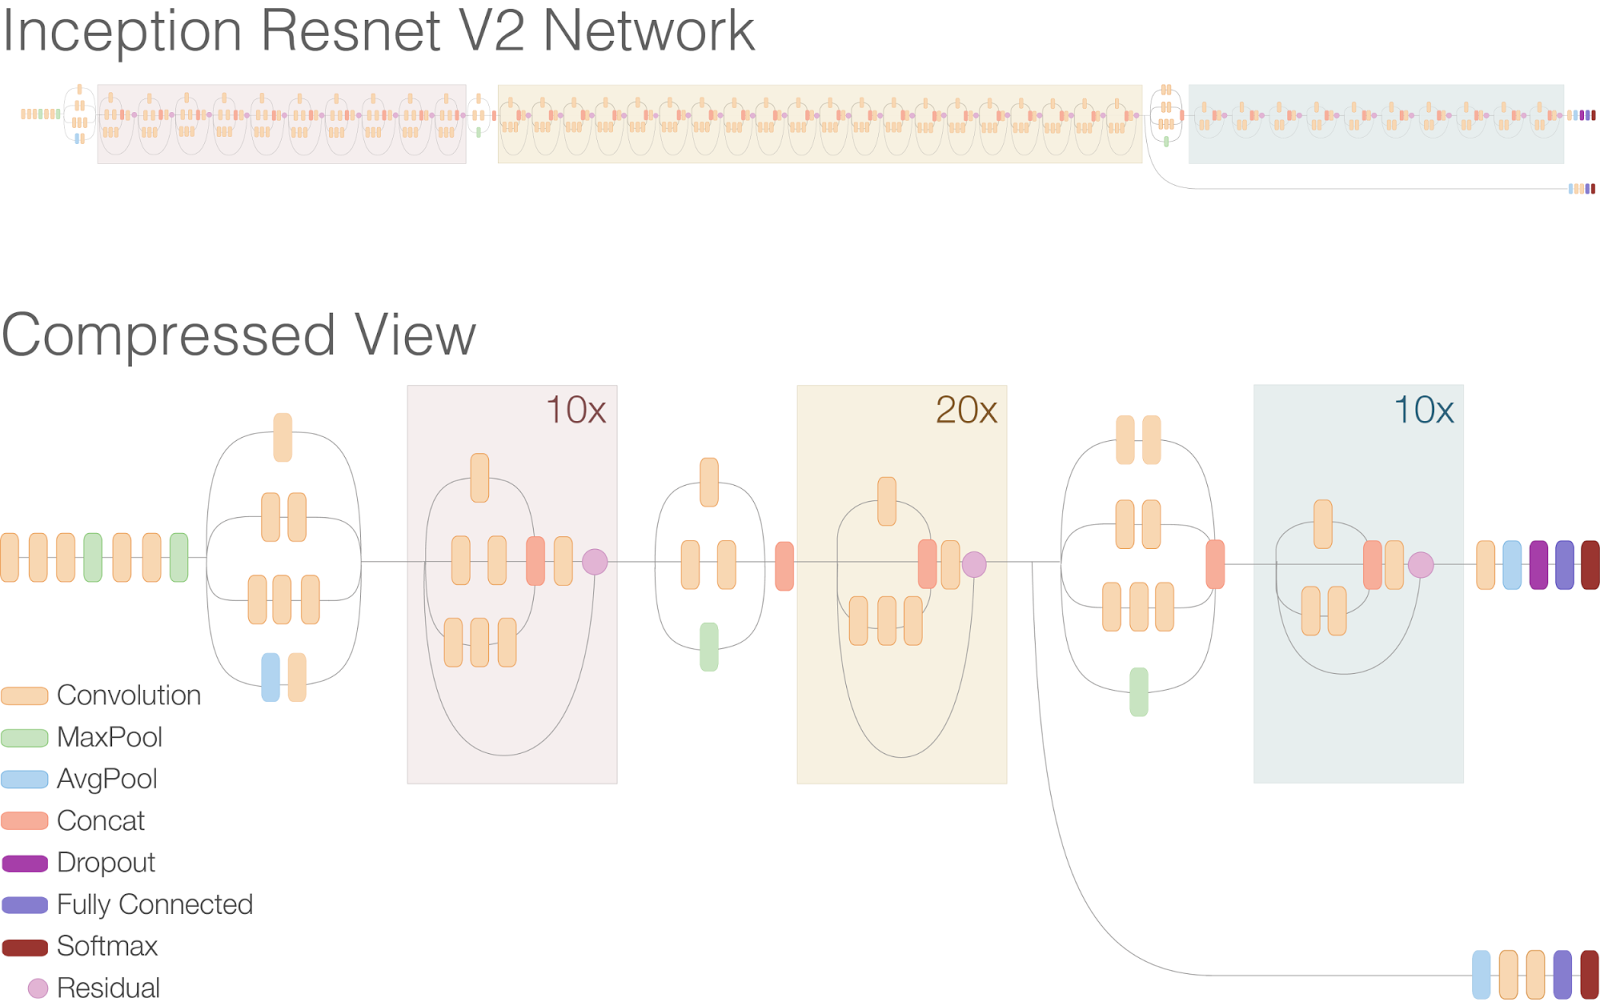
\includegraphics[width=.8\textwidth]{obrazky-figures/resnet.png}
    \caption[ResNet model structure]{ResNet model structure. \textit{Source: Google AI blog\,\footnotemark}}
    \label{fig:resnet}
\end{figure}
\footnotetext{\url{https://ai.googleblog.com/2016/08/improving-inception-and-image.html}}

\subsection{SqueezeNet}

SqueezeNet\,\cite{squeezenet} is a totally different architecture of deep neural networks than the previous mention. It introduced itself as an network with AlexNet accuracy, despite having half of the amount of parameters. It is designed to create small networks with fewer parameters than any other common network type.

Initially this network was released in 2016 as a Caffe implementation. Later it found its way into other frameworks and was hugely adopted in use cases with limited resources. Therefore it makes applications, which would require a model to be run on low-powered processing platforms like FPGAs and smartphones, available.

It is capable of optimizations like \textit{Deep Compression}\,\cite{compression}, which allows trained models to be compressed. In case of SqueezeNet it can reduce model size $10\times$.

\section{Experimental implementations of CapsNet}

Convolutional neural networks are already heavily established in the field, and since \textit{CapsNet} is a new and emerging architecture, it haven't proved itself in this particular field\,\cite{capsnet_comparative_perf}. Couple of different implementations exists, though only few are aiming for the facial recognition. However this architecture is the key delivery for this thesis, so it would be beneficial at least list the solutions and attempts to provide a reader more comprehensive view. First, we're will list the solutions to our problem and later focus better and more detail implementations which are more generic \textit{CapsNet}s or tackles different areas.

\subsection{CapsNet4Faces}

The only attempt I was able to locate at the time of publishing this thesis, which aims to solve the same problem as this thesis does. However the implementation\,\cite{capsnet4faces} seems incomplete and is based on the later mentioned \textit{Traffic sign classifier}\,\ref{ss:traffic_signs}. The basic description states 100\% accuracy although I was not able to replicate that and moreover all listed example Jupyter notebooks are faulty and do not contain expected outputs. In many places outdated results from Thibault Neveu's traffic sign classifier is shown. Despite the fact this solution is most likely not complete, it has to be listed, since it's the only publicly available solution using the same architecture found.


\subsection{CapsNet\,--\,Traffic sign classifier}
\label{ss:traffic_signs}

The most complete implementation of capsule network on a more complex problem than a MNIST data set. In this particular implementation\,\cite{capsnet_traffic}, the author Thibault Neveu focuses to create a classifier of German traffic signs. A network of 42 prediction capsules is able to assign correct label to a traffic sign with 98\% validation accuracy (97\% for testing). It follows similar architecture pattern as described above, at least for the \textit{encoder} part. The decoder is made differently, since a fully connected 3 layer decoding is not considered helpful for a image data in colour. Instead a convolutional decoder with resizing\,--\,up-scaling to nearest neighbour is used to provide reconstruction network. As per the documentation, this proved much more useful along with reduction in routing. The network is implemented in pure \textit{TensorFlow} framework. In our own solution later, we will use this network as a guidance and great inspiration for our work. The implementation is not very clean, though provide great insight into how one can manipulate and classify RGB data with emphasis on small feature size. We will borrow some visualization methods later in our example notebooks as well.

\subsection{CapsNet-Keras}

A thoughtful implementation\,\cite{capsnet_keras} of a capsule network in \textit{Keras} using \textit{TensorFlow} as back-end. Despite it sole focus on MNIST data set, it provides the most understandable and cleanest implementation of such network. As we will talk about later the chosen framework is a great advantage here. It follows very closely the implementation accented by Hinton\,\cite{capsule}. It features a 3 layer encoder with one composite primary capsules layer and one layer of prediction capsules, each per a digit. The architecture shown on figures\,\ref{fig:encoder} and\,\ref{fig:decoder} applies. As you may already recognize, that means this network has 10 prediction capsules, which greatly affects its size and keep it fairly small.


% \begin{table}[ht]
%     \centering
%     \begin{tabularx}{\textwidth}{X|ll|rrr}
%         & & & \multicolumn{3}{c}{Accuracy} \\
%         Name & Data set & License & Train & Validation & Test \\
%         \toprule
%         CapsNet4Faces & LFW & Apache 2.0 & 100\% & - & 93.7\% \\
%         Traffic sign classifier & Custom & Apache 2.0 & 99\% & 98\% & 97\% \\

%         \bottomrule
%     \end{tabularx}
%     \caption{Capsule networks comparison}
% \end{table}


\section{Frameworks}

Each of the previously mentioned solutions has something in common. They have used a AI framework or library of some sort. Writing neural networks from scratch is obviously a complex task, therefore there are many initiatives, which seeks to simplify and facilitate access to such complex structures. Let's list some of the most common ones and list some of their basic advantages and disadvantages.

\subsection{Torch and PyTorch}

Torch is a deep-learning and computational framework written in Lua. While very powerful, its design prevented from being adopted by users and researchers. The main problem was in usage of rather an exotic programming language, which created barrier for users. It is been decided to create a Python clone of the framework, which brought PyTorch\,\footnote{\url{https://pytorch.org/}} to existence. It was created by Facebook and released in 2007 under an open source license. One of its key features are dynamic computation graphs, which can serve well when processing inputs or outputs of variable length.

\begin{itemize}
    \item[$\boldsymbol{+}$] Many pluggable modules
    \item[$\boldsymbol{+}$] Easy to integrate different extensions
    \item[$\boldsymbol{+}$] Simple to define own layers
    \item[$\boldsymbol{+}$] Straightforward access to running code on GPU
    \item[$\boldsymbol{+}$] Offers dynamic computation graphs
    \item[$\boldsymbol{+}$] Broad community and wide audience
    \item[$\boldsymbol{+}$] Easier to inspect and monitor training of models
    \item[$\boldsymbol{+}$] Intuitive API
    \item[$\boldsymbol{-}$] Requires custom training code
\end{itemize}

\subsection{TensorFlow}

This library created by Google was designed as a replacement for their previous project called Theano. TensorFlow\,\footnote{\url{https://www.tensorflow.org/}} is a heavyweight framework written as a Python API in C/C++. It simplifies researcher's task in many ways better than other framework. For example it generates a computational graph and performs automatic differentiation. That means the user is not required to write a training code (back-propagation) every time, he's experimenting with a new network topology. Since this framework is backed by Google, it thrives in many different applications and can scale across devices. Many possibilities for applying saved models in different environment enables use of AI in mobile devices and even in web browsers. However it is broad possibilities and options make this framework hard to understand and for newcomers it can be confusing and too complex. Therefore an abstraction layer above TensorFlow had been created, but more about that in the \textit{Keras} subsection below.

\begin{itemize}
    \item[$\boldsymbol{+}$] Native Python and Numpy integration
    \item[$\boldsymbol{+}$] Automatic training code
    \item[$\boldsymbol{+}$] Broad community and wide audience
    \item[$\boldsymbol{-}$] Heavyweight frameworks
    \item[$\boldsymbol{-}$] A bit slower than PyTorch
\end{itemize}

\subsection{Caffe and Caffe2}

Caffe is another competition framework, which is widely popular among researchers. It started as a C/C++ port of Matlab's implementation of fast convolutional networks. It is mainly oriented on feed forward networks and image processing and is not intended for other deep learning application like text processing or 1D series data. Later on it became performance wise obsolete and community of Caffe developers decided to start from scratch and created a long-awaited successor Caffe2\,\footnote{\url{https://caffe2.ai/}}. Backed by Facebook, as their second deep learning toolkit after PyTorch, it provides more lightweight and scalable solution than before. It is main area of focus is enterprise grade production environments.

\begin{itemize}
    \item[$\boldsymbol{+}$] Great for image processing and feed-forward networks
    \item[$\boldsymbol{+}$] Automatic training code
    \item[$\boldsymbol{+}$] Lightweight
    \item[$\boldsymbol{+}$] BSD license
\end{itemize}

\subsection{Keras}

A modern abstraction layer above TensorFlow. Authors and users of TensorFlow suffered from heavy and complex code structures and when PyTorch appeared with their light and straightforward Python API, they have started adopting the same principles for the TensorFlow as well. Therefore a project named Keras\,\footnote{\url{https://keras.io/}} was created. It provides intuitive API inspired by Torch and while starting from TensorFlow it outgrown this base and spread across many deep learning libraries as its back-ends - Theano, Deeplearning4j, and CNTK. In addition to its high level abstraction over the back-ends, Keras also provides means to drill down and optimize and manipulate the underlying code.

\begin{itemize}
    \item[$\boldsymbol{+}$] Intuitive API
    \item[$\boldsymbol{+}$] Multiple back ends to choose from
    \item[$\boldsymbol{+}$] Lightweight
    \item[$\boldsymbol{+}$] Fast growing community
    \item[$\boldsymbol{+}$] Recognized as a standard Python API for neural networks
\end{itemize}

\section{Data Sets}

In order to better understand the nature of CCTV imagery, pictures in-the-wild and the source data we are about to work with, let's describe some commonly used databases of face images and face recognition data. It is crucial to understand the variety and differences between subjects captured on sample images, like their age, sex, and ethnicity. Also we need to pay attention to circumstances of the photo setup. That means for example consistency of resolution across samples, variety of poses and angles, etc.

\subsection{FDDB: Face Detection Data Set and Benchmark}

This data set provides annotations for Faces in the Wild\,\cite{fiw} database. FDDB\,\cite{fddb} lists coordinates for bounding boxes for over 5 thousands faces located on pictures from Faces in the Wild database. Usually multiple faces are located on a single picture. This data set can provide ground for face detection algorithms and therefore it can be benefited from in the first step of our implementation. For recognition of individuals, whom such face belongs to, another data set has to be used. A great accompanying data set can be the LFW, mentioned in next subsection.

\begin{table}[ht]
    \centering
    \begin{tabularx}{.8\textwidth}{l|X}
        \toprule
        Number of subjects & \num{5171} \\
        Total images &  \num{28045} \\
        Samples per subject & Varies, many have just one, others up to 40 \\
        Resolution & All kinds, even blurred faces \\
        License & Creative Commons \\
        \bottomrule
    \end{tabularx}
    \caption{FDDB data set metrics}
\end{table}

\subsection{LFW: Labeled Faces in the Wild}
\label{ss:lfw}

LFW\,\cite{lfw} provides labels for images from Faces in the Wild data set mentioned before. Therefore when used in conjunction with FDDB, this data set can provide a robust base for face recognition. The database spans many identities, though it lacks volume\,--\,many subjects have only one image in the data set. That does not provide enough coverage to train a network to recognize that individual.

\begin{table}[ht]
    \centering
    \begin{tabularx}{.8\textwidth}{l|X}
        \toprule
        Number of subjects & \num{5749} \\
        Total images & \num{13233} \\
        Samples per subject & Varies, many have just one, others up to 40 \\
        Resolution & 250 $\times$ 250 \\
        License & Creative Commons \\
        \bottomrule
    \end{tabularx}
    \caption{LWF data set metrics}
\end{table}

\subsection{The Extended Yale Face Database B}

Extended version of original Yale Face Database. The extension was provided by UCSD\,\cite{ext_yale_paper}. This database comprises of over \num{16000} images of 28 unique subjects. They are fitted to same size and resolution, covering various angles of the face. There are 9 poses provided for each person, each of them covering 64 different illumination condition. When compared to a large scale data set this database lacks volume, however it maintains consistency across its samples.

\begin{table}[ht]
    \centering
    \begin{tabularx}{.8\textwidth}{l|X}
        \toprule
        Number of subjects & 28 \\
        Total images & \num{16128} \\
        Samples per subject & 576 \\
        Poses & 9 \\
        Resolution & $168 \times 192$ pixels \\
        License & Free to use for research purposes\\
        \bottomrule
    \end{tabularx}
    \caption{Extended Yale Face Database B metrics}
\end{table}

\subsection{SCface - Surveillance Cameras Face Database}

A face database originated from University of Zagreb. Quality data set of surveillance-like face images. It aims to simulate a CCTV captured images by maintaining an uncontrolled indoor environment. Each of 130 subjects is captured by up to 8 video surveillance cameras. Some of them even capable of IR capturing. Each camera produces images of different resolution and sharpness. Cameras are also set in different angles against the subject. SCFace\,\cite{scface} mimics real-world circumstances and use cases of CCTV, therefore this data set can be used to train robust solutions for face recognition targeting CCTV and surveillance cameras.

A disadvantage is the size of this data set, where we can find \num{4160} image samples only. When compared to large-scaled data set like the VGGFace and VGGFace2 mentioned in next subsection, this data set lacks volume. Also the variety of subjects is not robust enough in comparison to other data set. As said, SCFace captures 130 subjects. Most of them are of the same sex, all of the same ethnicity.

\begin{table}[ht]
    \centering
    \begin{tabularx}{.8\textwidth}{l|X}
        \toprule
        Number of subjects & 130 \\
        Total images & \num{4160} \\
        Samples per subject & Fixed amount of 32 images per person \\
        Resolution & Varies, 3 different sizes \\
        License & Custom, research purpose only \\
        \bottomrule
    \end{tabularx}
    \caption{SCFace data set metrics}
\end{table}

This database is available for research purposes and upon written request to the authors.

\subsection{VGGFace2}

Visual Geometry Group produced a second iteration of their face recognition data set\,\cite{VVGFace2}. This is one of the widest data sets which are publicly available. It provides a wide-scale data for face recognition for over 9000 different identities. Distribution of individuals varies though, with minimal 87 images up to 843 per identity. Average number of images per subject is 362. The data set contains over \num{3.3} million of images in total. Subjects varies in ethnicity, age and profession, while the images varies in angles or poses. Collection of such vast amount of images is a product of web scraping, so the images might not always be consistent with definition of pictures in-the-wild.

The data set is made available under Creative Commons license\,\footnote{\url{https://creativecommons.org/licenses/by-sa/4.0/}}, therefore it is available for broad use to any project.

\begin{table}[ht]
    \centering
    \begin{tabularx}{.8\textwidth}{l|X}
        \toprule
        Number of subjects & \num{9294} \\
        Total images & \num{3311286} \\
        Samples per subject & Varies, 87--843 per subject \\
        Resolution & Varies, many different sizes \\
        License & Creative Commons \\
        \bottomrule
    \end{tabularx}
    \caption{VGGFace2 data set metrics}
\end{table}

This project also provides sample models trained on their data set. However, the provided example pre-trained neural network models are not the sole representation of its usage. Many popular face recognition models are trained on this data set. For example FaceNET, mentioned before\,\ref{ss:facenet}, can be seen as one of the popular projects which benefits from this data set.

\subsection{MSCeleb}

This data set is provided by Microsoft company and various challenges and competitions were held against it. Similarly to the previous one, MSCeleb\,\cite{msceleb} is a large scale data set, though oriented specifically on celebrities. Each challenge announced by their researcher team is backed by a specific subset of the data set. These selections are usually oriented on certain aspects of face recognition, therefore can be proven valid for use case covered in this thesis.

Subjects vary in all desired aspects and images provide enough variety in poses and background noise.

\begin{table}[ht]
    \centering
    \begin{tabularx}{.8\textwidth}{l|X}
        \toprule
        Number of subjects & \num{99892} \\
        Total images & \num{8456240} \\
        Samples per subject & Varies, average 85 per entity \\
        Resolution & Varies, up to 300 $\times$ 300 \\
        License & Research purposes only \\
        \bottomrule
    \end{tabularx}
    \caption{MSCeleb data set metrics}
\end{table}

\subsection{CelebA}

CelebA\,\cite{celeba} is another large scale database of faces. The focus is on celebrities faces, the same as in the MSCeleb data set. Pictures cover wide variety of poses and background noises. Each image is provided with 5 landmarks locations and 40 binary attributes.

Subjects vary in ethnicity, age, sex as well as in appearance. Data set includes faces with facial hair, poses and with different emotions.

\begin{table}[ht]
    \centering
    \begin{tabularx}{.8\textwidth}{l|X}
        \toprule
        Number of subjects & \num{10177} \\
        Total images & \num{202599} \\
        Samples per subject & Varies \\
        Resolution & Varies \\
        License & Research purposes only \\
        \bottomrule
    \end{tabularx}
    \caption{CelebA data set metrics}
\end{table}

\subsection{Aligned Face Dataset from Pinterest}
\label{ss:pins}

Aligned Face Dataset from Pinterest (PINS) is a custom data set available on Kaggle\,\cite{pins}. It provides normalized, aligned and feature centred image data collected from Pinterest and processed via \textit{dlib}. The image distribution is not strictly uniform, although it provides at least 100 images per identity. The only drawback is that images listed are not always in-the-wild. Many times it include stages photos, many of them post processed and modified. Therefore despite interesting metrics, the data set proved unusable because of it great great inconsistency within each identity domain.

\begin{table}[ht]
    \centering
    \begin{tabularx}{.8\textwidth}{l|X}
        \toprule
        Number of subjects & \num{100} \\
        Total images & \num{10770} \\
        Samples per subject & Varies \\
        Resolution & Varies \\
        License & Research purposes only \\
        \bottomrule
    \end{tabularx}
    \caption{PINS data set metrics}
\end{table}
